%%
% Please see https://bitbucket.org/rivanvx/beamer/wiki/Home for obtaining beamer.
%%



\documentclass[hyperref={pdfpagelabels=false},xcolor=dvipsnames]{beamer}
\usepackage{lmodern}
%\mode<presentation>{
%\usetheme{Copenhagen}
\usecolortheme{dove}
\setbeamertemplate{footline}[page number]
%\setbeamertemplate{navigation symbols}{}
%}

\usetheme{Singapore}
%\usecolortheme[named=Gray]{structure}
\usepackage[utf8]{inputenc}
\usepackage[ngerman]{babel}
\usepackage{graphicx}
%\usepackage{booktabs}
\setbeamertemplate{navigation symbols}{}




\setbeamercolor{normal text}{fg=darkgray}
\setbeamercolor{frametitle}{fg=darkgray}

\usebeamercolor*{normal text}
\usebeamercolor*{frametitle}


\newcommand*\mi{ \item[\color{gray}\scalebox{1.2}{\textbullet}]}


\title{VLAN und VPN}
\author{KL}
\institute{Fernuniversität Hagen}
\date{WS 18/19}





\begin{document}

\begin{frame}
	\titlepage
\end{frame}
%%%%%%%%%%%
\begin{frame}
	\frametitle{Inhalt}
	\tableofcontents	
\end{frame}
%%%%%%%%%%%
\section{Einleitung}
\begin{frame}
	\frametitle{IT-Sicherheit in kleinen Unternehmen} Studie des WIK: 	
	\begin{itemize}
		\mi 64\% derkleinen Unternehmen finden IT-Sicherheit sehr wichtig
		\mi $20\%$ haben eine Sicherheitsanalyse durchgeführt
		\mi $94\%$ haben PC-Arbeitsplätze mit Internetzugang
		\mi $75\%$ nutzen mobile Endgeräte (Smartphone, Tablet, Notebook)
		\mi 31\% nutzen VPN
		\mi 53\%	waren von Virenangriffen betroffen
	\end{itemize}
	
\end{frame}
%%%%%%%%%%%
\section{Sichere Netzwerkarchitektur}

\begin{frame}
	\frametitle{Grundarchitektur eines sicheren Netzwerkes}
	\begin{figure}
	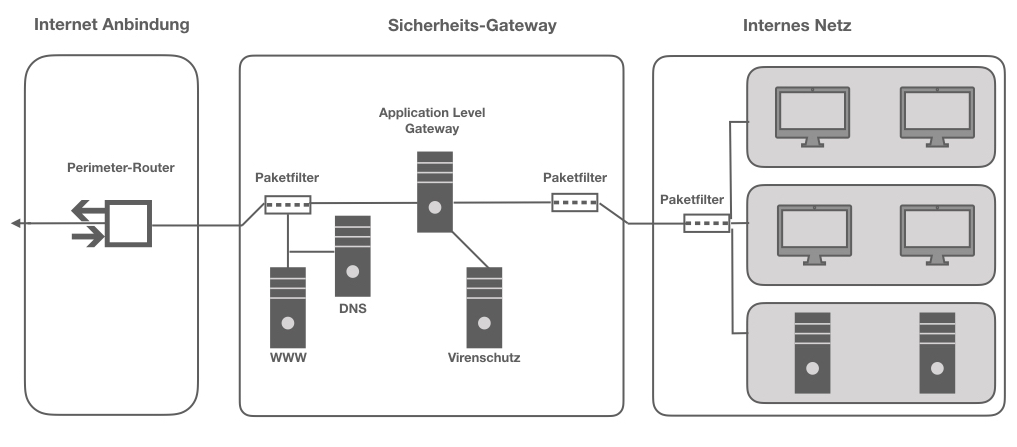
\includegraphics[width=\textwidth]{grundarchitektur.jpeg}	
	\end{figure}
		
\end{frame}
%%%%%%%%%%%%
\begin{frame}

	\frametitle{Grundarchitektur für kleine Unternehmen mit hohem Schutzbedarf}
	
	\begin{figure}
	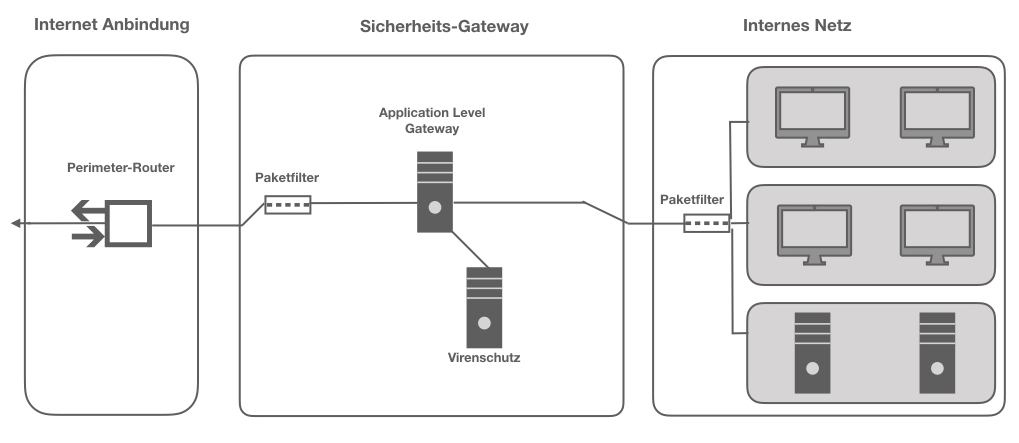
\includegraphics[width=\textwidth]{klUnternehmnorm}	
	\end{figure}
		
\end{frame}


\begin{frame}

	\frametitle{Grundarchitektur für kleine Unternehmen mit normalem Schutzbedarf}
	
	\begin{figure}
	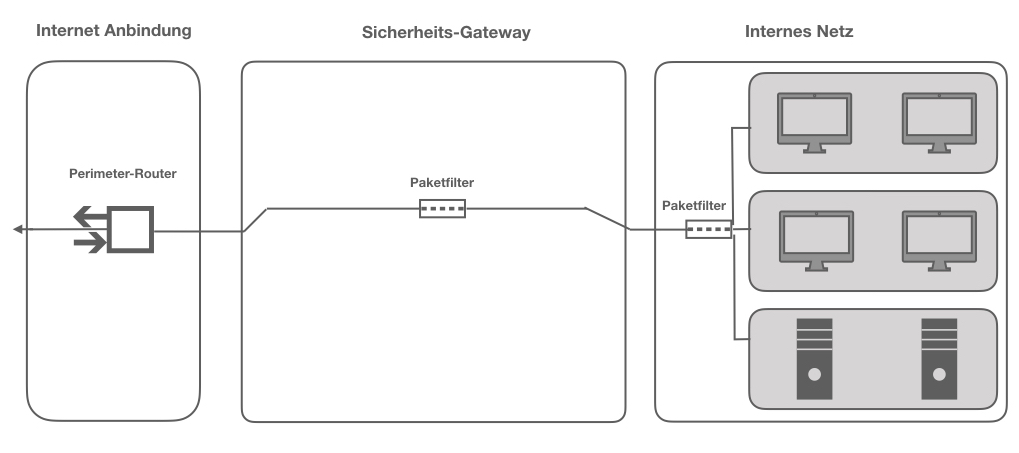
\includegraphics[width=\textwidth]{klUnternHoch}	
	\end{figure}
		
\end{frame}

%%%%%%%%%%%%%%
%%%%%%%%%%%%%%
\section{Virtuelle lokale Netzwerke VLAN}
%
\begin{frame}
	\frametitle{Virtuelle lokale Netze VLAN}
	\begin{itemize}
		\mi  physische LANs in logische Einheiten unterteilen
		\mi verschiedene physische Netze virtuell zu verbinden
		\mi Kostenersparnis $\leftarrow$ weniger Hardware
		\mi Hohe Flexibilität
		\mi Verkleinerung der Broadcastdomäne
		 
		
	\end{itemize}

\end{frame}

%%%%%%%%%%%%%%
\begin{frame}

	\frametitle{Portbasiertes VLAN}
	
	\begin{figure}
	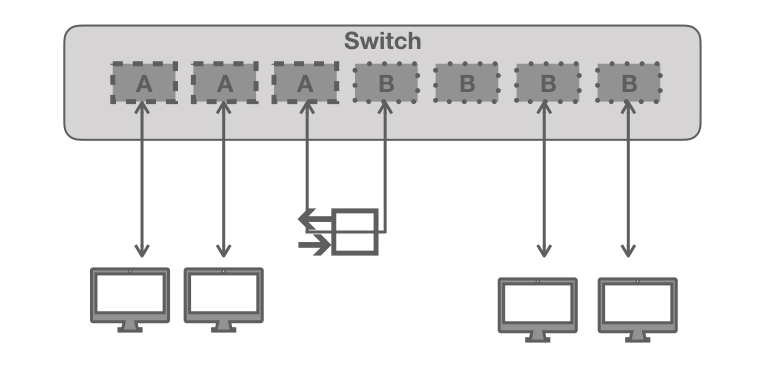
\includegraphics[width=\textwidth]{vlan.001.jpeg}	
	\end{figure}
		
\end{frame}

%%%%%%%%%%%%%%%
\begin{frame}
	\frametitle{Tagged VLAN}
		\begin{figure}
	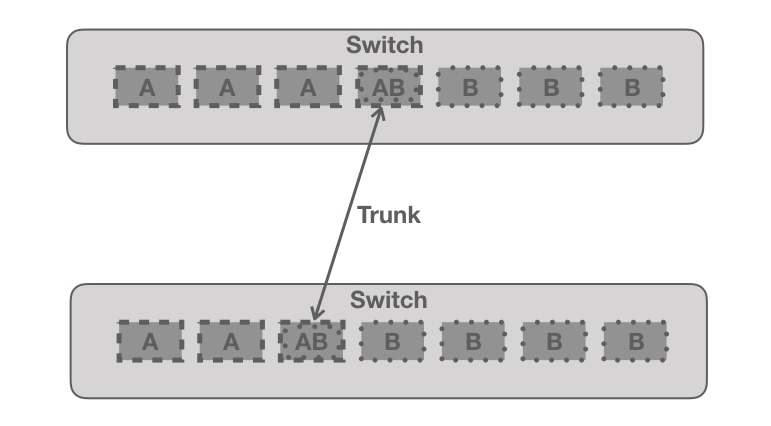
\includegraphics[width=\textwidth]{vlan.002.jpeg}	
	\end{figure}	
\end{frame}

%%%%%%%%%%%%%%%%


%%%%%%%%%%%%%
%%%%%%%%%%%%%
\section{Virtuelle Private Netze VPN}

\begin{frame}
	
\end{frame}
%%%%%%%%%%%%%

\begin{frame}
	
\end{frame}

%%%%%%%%%%%%%
%%%%%%%%%%%
\section{Ausblick}

\begin{frame}
	
\end{frame}


\end{document}



